% previousresearch.tex

% Previous Research
\section{Previous Research and Background}
\label{sec:previousresearch}
System simulators are abundant and exist in corporate~\masccite{magazines:bohrer:2004}, academic~\masccite{journals:rosenblum:1995}, and open-source variations~\masccite{inproceedings:bellard:2005}.
Such platforms, like Simics, are used for many purposes including thermal control strategies in multicores~\masccite{inproceedings:bartolini:2010}, networking timing analysis~\masccite{journals:ortiz:2009}, web server performance evaluation~\masccite{journals:villa:2005}, and to simulate costly hardware financially unfeasible to researchers~\masccite{journals:alameldeen:2003}.

Lagar-Cavilla et al. present VMGL, an OpenGL virtualization solution that can accelerate OpenGL~$1.5$ up to two orders of magnitude in comparison to software rasterization~\masccite{inproceedings:lagarcavilla:2007}.
The solution runs the OpenGL library and GPU driver on the VMM host, and utilizes network transport to relieve OpenGL commands between target and host systems.
VMGL was evaluated in WMware Workstation and Xen VMMs.

\begin{figure}
\centering
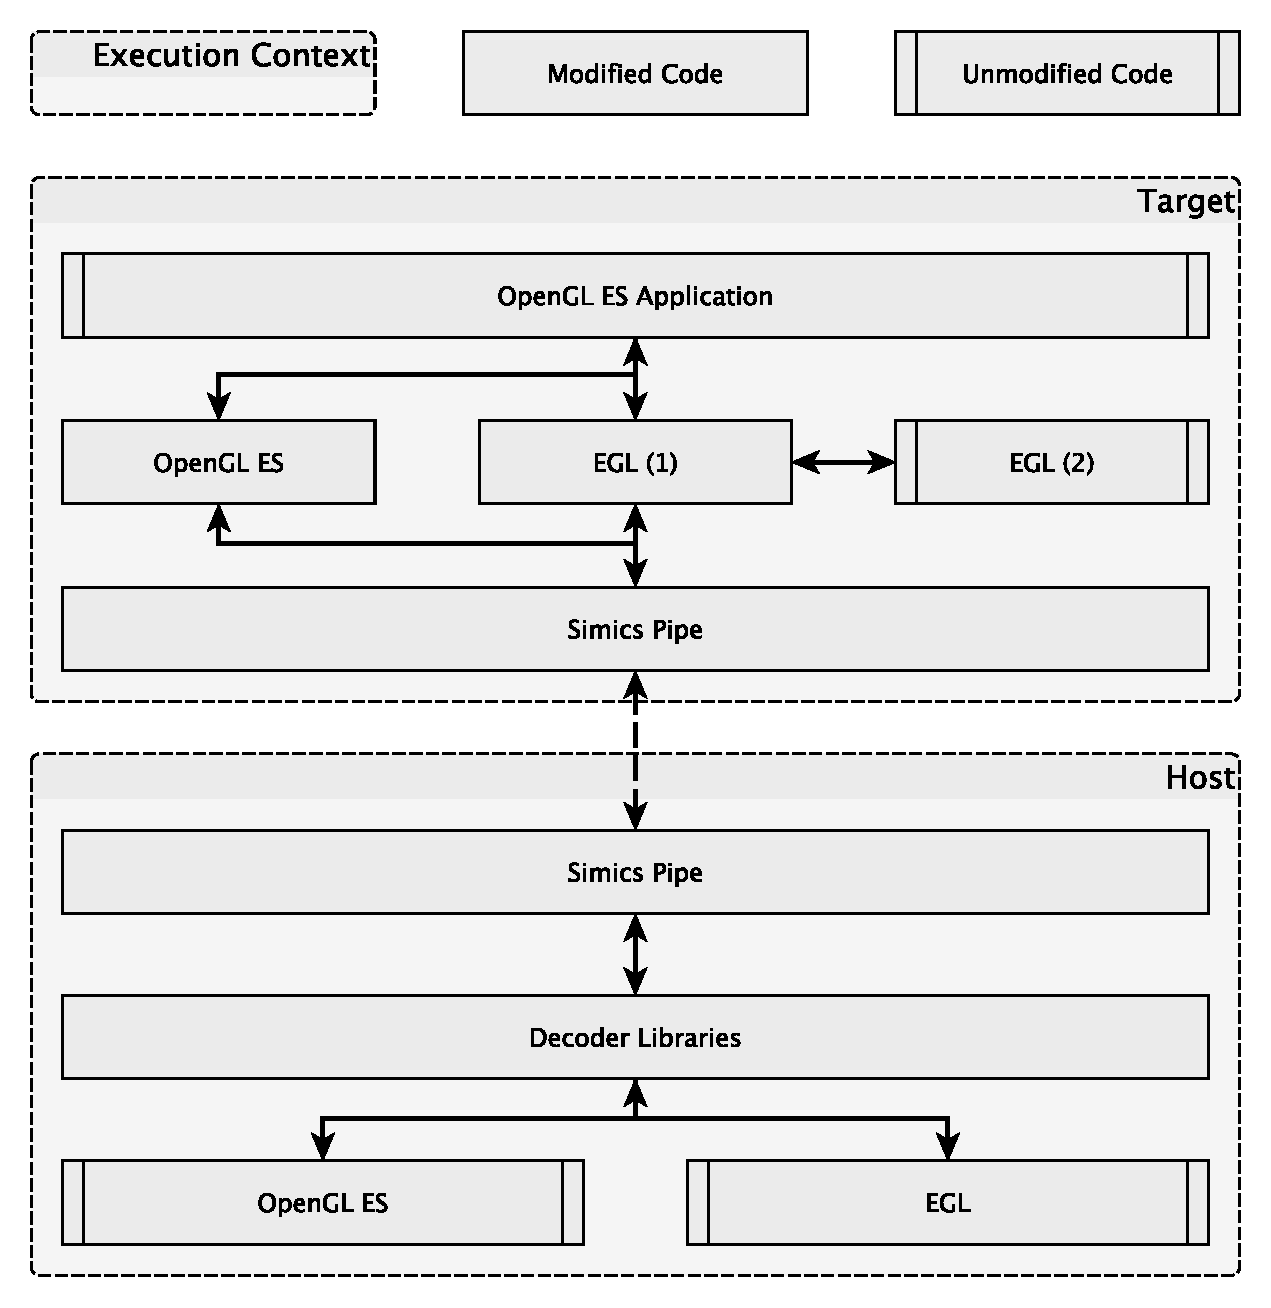
\includegraphics[width=\linewidth]{img/yedoverview.pdf}
\caption{Overview of paravirtualized graphics in Simics.}
\label{fig:overview}
\end{figure}
